\section{Introduction}


Understanding the performance of virtualized multi-tier applications is crucial for efficient cloud infrastructure management. Several enterprises, especially large ones that have already invested in their own infrastructure over the years are looking at setting up private clouds within their organizational boundaries 
to reap the benefits of cloud computing technologies leveraging such investments. 

Virtualization renders prominent accessibility for vital applications and streamlines application preparation and movements. CLOUD stands for Computing Location independent Online Utility which is a useable, on-Demand service that permits users access and occupy resources on internet devices connected to local, remote and other connection. Cloud computing is defined as an ''Internet based computing,'' where different utilities like storage, servers and applications are handled by a separate entity's computers and devices through the Internet [4]. 

% quote
\begin{quote}
  ``It (CLOUD) provides the guest user with the elements needed to execute his request, while it gives the provider the ability to be housing different guests without risking the security and integrity of data.''[7]
\end{quote}
The use of VM in Cloud Computing has become very popular nowadays. In fact, it is becoming more and more common in virtualization approaches due to its simplest basis of dividing a physical computer into many isolated machines, allowing the user (guest) to work on different environments (OS, applications ...) using the same devices. This virtualization comes however with some security threats, and the most evident question one can asks himself in this situation is ''Once one of the VM environments gets infected, will it impact all my data's security and privacy? Will this infection be able to threaten even my personal data that I did not share on the cloud?''. Thus, Virtualization comes with several challenges. In this paper, we will discuss the following:
% itemize
\begin{itemize}
\item The existing virtualization techniques, including process 
virtualization, OS virtualization and system virtualization.
\item Challenges in virtualizing different types of resources, 
such as CPU, memory and I/O devices.
\item Why virtualization is the enabling technology for the cloud ecosystem
\end{itemize}

% Head 1
\section{VIRTUALIZATION TECHNIQUES}

% Head 2
\subsection{SERVER VIRTUALIZATION}

Server virtualization is the most active segment of the virtualization industry featuring established companies such as VMware, Microsoft, and Citrix. With server virtualization one physical machine is divided many virtual servers. At the core of such virtualization is the concept of a hypervisor (virtual machine monitor). A hypervisor is a thin software layer that intercepts operating system calls to hardware. Hypervisors typically provide a virtualized CPU and memory for the guests running on top of them. The term was first used in conjunction with the IBM CP-370. Hypervisors are classified as one of two types:

Type 1 : This type of hypervisor is also known as native or bare metal. They run directly on the hardware with guest operating systems running on top of them. Examples include VMware ESX, Citrix XenServer and Hyper-V.

Type 2 : This type of hypervisor runs on top of an existing operating system with guests running at a third level above hardware. Examples include VMware Workstation and Parallels Desktop.

Related to type 1 hypervisors is the concept of paravirtualization.

% Head 4
\paragraph{Paravirtualization}

Paravirtualization is a technique in which a software interface that is similar but not identical to the underlying hardware is presented. Operating systems must be ported to run on top of a paravirtualized hypervisor. Modified operating systems use the "hypercalls" supported by the paravirtualized hypervisor to interface directly with the hardware. The popular Xen project makes use of this type of virtualization. Starting with version 3.0 however Xen is also able to make use of the hardware assisted virtualization technologies of Intel (VT-x) and AMD (AMD-V). These extensions allow Xen to run unmodified operating systems such as Microsoft Windows.

\subsection{OPERATING SYSTEM VIRTUALIZATION}

Operating system virtualization provides application-transparent virtualization to users by decoupling applications from the OS. The OS virtualization technique offers granular control at the application level by facilitating the transparent migration of individual applications. The finer granularity migration offers greater flexibility, resulting in reduced overhead.

OS virtualization can also be used to migrate critical applications to another running operating system instance. Patches and updates to the underlying operating system are done in a timely way, and have little or no impact on the availability of application services. The processes in the OS virtualized environment are isolated and their interactions with the underlying OS instance are monitored.

% description
\begin{description}
\item[Advantages of OS virtualization]
\item OS virtualization usually imposes little or no overhead.

OS Virtualization is capable of live migration.

It can also use dynamic load balancing of containers between nodes and a cluster.

The file level copy-on-write (CoW) mechanism is possible on OS virtualization which makes easier to back up files, more space-efficient and simpler to cache than the block-level copy-on-write schemes.
\end{description}


\subsection{PROCESS VIRTUALIZATION}
\label{sec:sim}

Process Virtualization technology ensures that a Task is executed exactly as if it is being executed on the computer that initiated the Job (Initiating Machine), regardless of the remote Agent's file system, installation base, and environment. It does not require any installations on remote agents, and does not require files to be copied from Initiating Machine. Process Virtualization ensures that files (including DLLs and others) required by the remote process are transferred automatically and transparently from Initiating Machine to Helper Machines.

For process virtualization, the VM interfaces with the single process. The running application sees "virtual machine" as address space, registers and instruction set. Examples for this are:
% enumerate
\begin{enumerate}
\item Multiprogramming.
\item Emulation for binaries.
\item High level language VMMs.
      \begin{enumerate}
      \item JVM.
      \end{enumerate}
\end{enumerate}
Figure~\ref{fig:one} shows a basic outline of how virtualization is carried out.
% * <rajvi23t@gmail.com> 2018-05-02T03:04:26.362Z:
%
% ^.
% Figure
\begin{figure}
  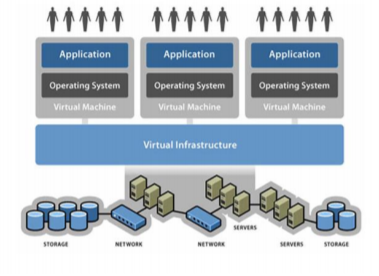
\includegraphics{snip}
  \caption{Mechanism for Virtualization.[7]}
  \label{fig:one}
\end{figure}


\section{Virtualization Challenges}
There are varied challenges associated with virtualizing resources such as CPU, memory and I/O devices. A brief overview of the same is provided below:
\subsection{CPU Virtualization}
\label{sec:vir}
The trap-and-emulate approach used
by VT hardware generates a lot of traps, and traps are very expensive on modern
hardware because they ruin CPU caches, TLBs, and branch prediction tables internal
to the CPU. In contrast, when sensitive instructions are replaced by calls to
hypervisor procedures within the executing process, none of this context-switching
overhead is incurred.  For this reason, some type 1 (and type 2)
hypervisors do binary translation for performance reasons, even though the software
will execute correctly without it.

% description
\begin{description}
\item[Main challenges for CPU virtualization]
\item Privileged Instructions : Handling architecture imposed instruction privilege levels.

 Performance Requirements : Holding down the cost of VMM activities.
\end{description} 

\subsection{Memory Virtualization}
\label{sec:vir}
Memory Virtualization introduces a way to decouple memory from the processor, AND, from the server to provide a shared, distributed or networked function. Modern operating systems nearly all support virtual memory, which is basically a mapping of pages in the virtual address space onto pages of physical memory. This mapping is defined by (multilevel) page tables. Typically the mapping is set in motion by having the operating system set a control register in the CPU that points to the top-level page table. Virtualization greatly complicates memory management.

A big challenge is to minimize page faults. Page faults are always expensive, but especially so in virtualized environments, because they lead to so-called VM exits. A VM exit is a situation in which the
hypervisor regains control. Let us consider what the CPU needs to do for such a VM exit. First, it records the cause of the VM exit, so the hypervisor knows what to do. It also records the address of the guest instruction that caused the exit. Next, a context switch is done, which includes saving all the registers. Then, it loads the
hypervisors processor state. Then the hypervisor can start handling the page fault, which was expensive to begin with. It also needs to reverse these steps. The whole operation may take tens of thousands of cycles. This proves to be a significant and hindering overhead for the virtualization process. Thus, efficiently managing multiple memory spaces and avoiding page faults is important.

% description
\begin{description}
\item[Main challenges for Memory virtualization]
\item Memory Management : Managing multiple address spaces efficiently.

 Reducing Page Faults/VM exits : Costly operations.
\end{description} 
 
\subsection{I/O Virtualization}
\label{sec:vir}
In many systems, a nontrivial performance penalty is associated with indirection. The same can be true for virtualized I/O, since I/O operations must conceptually traverse two separate I/O stacks: one in the guest managing the virtual hardware and one in the hypervisor managing the physical hardware. The longer I/O path affects both latency and throughput, and imposes additional CPU load. Indeed, I/O-intensive workloads on some early virtualization systems suffered a virtualization penalty larger than a factor of two. Since then, further research, optimizations, and hardware acceleration have reduced this penalty into the noise for an impressive set of demanding production workloads. Somewhat counterintuitively, virtualized systems have even outperformed native systems on the same physical hardware, overcoming native scaling limitations by instead running several smaller VM instances in a scale-out configuration.

The majority of server virtualization deployments are configured for high availability and, as a result, are heavily reliant on shared networked storage. As the number of VMs on a physical host increases, shared storage can quickly lead to storage I/O bottlenecks.

% description
\begin{description}
\item[Main challenges for I/O virtualization]
\item  Handling I/O requests from multiple operating
systems. 

 DMAs: Absolute memory addresses used
 
 Bottlenecks associated with use
\end{description} 
% Table
\begin{table}%
\caption{Challenges to Virtualization}
\label{tab:one}
\begin{minipage}{\columnwidth}
\begin{center}
\begin{tabular}{ll}
  \toprule
  CPU   & \\
  1     & Handling privilege levels\\
  2  & Minimizing cost of VMM activities\\
  Memory     & \\
  1    & Multiple address spaces or page tables\\
  2   & Reducing VM exits\\
  I/O       & \\
  1     & Requests from multiple OSs\\
  2 & Use of absolute memory addresses\\
  3     & bottlenecks due to sharing\\
  \bottomrule
\end{tabular}
\end{center}
\bigskip\centering
\footnotesize\emph{Source:} Self compiled.

 \emph{Note:} This is a table footnote.
\end{minipage}
\end{table}%


\section{CLOUD ECOSYSTEM AND VIRTUALIZATION}

Cloud computing is becoming popular as virtualization power, distributed computing with server cluster
and increase in the availability of broadband internet assessing is increasing.
The IT world is looking forward for the services provided by cloud computing thus boosting up the
development of cloud computing.
NIST [8] has defined cloud as ''Cloud computing is a model for enabling ubiquitous, convenient, on demand
network access to a shared pool of configurable computing resources (e.g., networks, servers, storage,
applications, and services) that can be rapidly provisioned and released with minimal management effort or
service provider interaction''. 

\subsection{DEFINITION AND SCOPE}

% Head 4
\paragraph{Definition: }

Cloud computing is the outcome of grid computing, utility computing and automatic computing.
Cloud is a parallel and distributed computing system which consists a set of inter connected and virtualized
computers which gives one or more unified computing resources based on the requirements between service
providers and service consumers[3].

Cloud computing is on demand pay-as-use i.e billing is done based on the usage of the customer which
downs the operational and capital cost. Users can access applications which are present outside the working site
which can access remote applications through internet connection devices. By this, computer resources can be
efficiently used and consume less computing power and resources are shared cooperatively.
Cloud computing services are first offered by Amazon, Google, Microsoft and now many are existing.
These services are used by software industries, government sectors, and health care sectors and in many more
fields.
The main power of cloud computing lies in the way data is stored, how it is transmitted and accessed. A
virtualized platform with management capabilities like availability, automated load balancing and fault
tolerance reduces infrastructure cost and maintenance cost.

\subsection{ELEMENTS OF CLOUD}
Clients: Users like computers, laptops, tablets computers mobile phones or PDA's.

Data Centers: These are a collection of servers where the application is hosted. Virtualization is done where
multiple instances of virtual servers are created.

Distributed Server: Servers which reside non locally which are geographically far.

There are three typed of cloud services:
\begin{description}
\item[Saas]
\item 'Software as a Service' is the model in which an application is hosted as a service to customers who access through internet. Users can access their application anywhere if they are connected to internet. Some of the applications are CRM (customer Resource Managing), accounting, web content managing.
\end{description}
\begin{description}
\item[PaaS]
\item  Platform as a Service. This is another application delivery model which provides resources required to
build application and services completely from internet without purchasing.Developers can design, develop, test and deploy and host applications. More services are like team collaboration, web service integration, DB integration.
\end{description}
\begin{description}
\item[IaaS]
\item  Infrastructure as a service. This provides the required hardware so that users can put anything they
required. IaaS allows renting of resources like server space, cpu cycles, network equipments, memory and
storage space.
\end{description}

\subsection{VIRTUALIZATION IN CLOUD COMPUTING}
Virtualization technology makes cloud computing environment easily to manage the resources. It abstracts and
isolates the underlying hardware, and networking resources in a single hosting environment. It increases the security of cloud computing by protecting both the integrity on guest virtual machine and
cloud components virtualized machines can be scaled up or down on demand and can provide reliability. It
provides resource sharing, high utilization of pooled resources, rapid provisioning, workload isolation.
The recent trends in virtualization are consolidation of data centers thus reducing the managing cost.

Apart of its benefits it has some drawbacks like managing virtual resources is critical and migrating services of these resources are difficult in achieving high availability.
If one server fail VM will be restarted on the other virtualized server in resource pool restoring the required
services with minimum service interruption.
Virtual resources are critical for managing and data monitoring. Running applications with high utilization and
availability is a challenging issue. 

\paragraph{Security Perspective:} Hypervisor controls all the guest systems. As the operating system number increases managing is difficult these leads to security issues. If a hacker gets control over the hypervisor he can control the guest systems by knowing the behavior of the system which causes data processing damage. Advanced protection system is to be developed to monitor the activities of the guest Virtual machine[3].
Data loss, data security and inconvenience to access the data are
some of the major problems that users face but with the use of cloud
computing these problems can be resolved easily. Some of the major
future aspects are:

a. Migration time will become negligible

b. Data is secured and data loss is minimized

c. One user-many devices relationship

\section{CONCLUSION}
We have discussed the nuances of virtualization and have developed its relationship with the cloud. To have physical and virtual controls in the cloud environment one must protect data by implementing strong
encrypting techniques using secure connections and applying data loss prevention policies[5].
Access control policies are to be established and client identities are to be checked.
Datacenter platforms, infrastructure and client devices are to be secured by trusted computer policies.
Enable secure migration from private cloud environment to public cloud providers.

Virtualization technology offers important utilities which make it an indispensable tool that can be used in a large number of applications. These are not limited to server consolidation, application sandboxing, access to  different types of hardware and operating systems, debugging, etc. There are different techniques that Virtual Machine ware is pursuing to make performance of virtualization better over time. The idea of cloud computing is getting more preferred and it has a long way to be developed. Cloud computing provides lots of benefits to the users and makes resource management much easier for the user. We discussed the challenges associated with virtualization as well as the cloud development cycle. The scope has also been presented. This survey paper proves that much more in-depth research can, and hence should, be pursued in these designated areas.

% Appendix
\appendix

\begin{acks}

The author would like to thank Dr. Jia Rao at The University of Texas at Arlington's Computer Science and Engineering Department for providing specifications and guidance regarding the topic. His assistance in routing the author towards similar research papers and books have helped in the realization of this paper. 



\end{acks}

% Bibliography
\bibliographystyle{ACM-Reference-Format}
\bibliography{REFERENCES}

[1] AMD. AMD64 Virtualization Codenamed ''Pacifica'' Technology:
Secure Virtual Machine Architecture Reference Manual, May 2005.

[2] AMSDEN, Z., ARAI, D., HECHT, D., HOLLER, A., AND SUBRAHMANYAM,
P. VMI: An interface for paravirtualization. Ottawa Linux
Symposium (2006).

[3] DEITEL, H. M. An introduction to operating systems (2nd ed.).
Addison-Wesley Longman Publishing Co., Inc., Boston, MA, USA,
1990.

[4] HENNESSY, J. L., AND PATTERSON, D. A. Computer architecture:
a quantitative approach. Morgan Kaufmann Publishers Inc., San
Francisco, CA, USA, 2002.

[5] INTEL CORPORATION. Intel
R Virtualization Technology Specification
for the IA-32 Intel
R Architecture, April 2005

[6] POPEK, G. J., AND GOLDBERG, R. P. Formal requirements for
virtualizable third generation architectures. Commun. ACM 17, 7
(1974), 412-421.

[7] SILBERSCHATZ, A., AND PETERSON, J. L., Eds. Operating systems
concepts. Addison-Wesley Longman Publishing Co., Inc., Boston,
MA, USA, 1988.

[8] SMITH, J. E., AND NAIR, R. Virtual machines: versatile platforms for
systems and processes. Morgan Kaufmann Publishers, San Francisco,
CA, USA, 2005.

[9] KARGER, P. A., ZURKO, M. E., BONIN, D. W., MASON, A. H.,
AND KAHN, C. E. A vmm security kernel for the vax architecture. In
IEEE Symposium on Security and Privacy (1990), pp. 2-19.

[10] LEVASSEUR, J., UHLIG, V., CHAPMAN, M., CHUBB, P., LESLIE,
B., AND HEISER, G. Pre-virtualization: Slashing the cost of
virtualization. Technical Report 2005-30, Fakultat fur Informatik,
Universitat Karlsruhe (TH), Nov. 2005.

[11] MCGHAN, H., AND O'CONNOR, M. Picojava: A direct execution
engine for java bytecode. Computer 31, 10 (1998), 22-30.

[12] NEIGER, G., SANTONI, A., LEUNG, F., RODGERS, D., AND UHLIG,
R. Intel virtualization technology: Hardware support for efficient
processor virtualization. Intel Technology Journal 10, 3 (2006).

[13] OSISEK, D. L., JACKSON, K. M., AND GUM, P. H. ESA/390
interpretive-execution architecture, foundation for VM/ESA. IBM
Systems Journal 30, 1 (1991), 34-51.

